\documentclass{beamer}\mode<presentation>{\usetheme{AMSCesenaPurpleAndGold}}
%\documentclass[presentation]{beamer}\mode<presentation>{\usetheme{AMSCesenaPurpleAndGold}}
%%%%

\usepackage{sd-lab-async-programming}
\usepackage{my-listings}

\title[Async Programming 101]{Asynchronous Programming 101}
%
\subtitle[SD]
{Distributed Systems / Hands-on\\\scriptsize Sistemi Distribuiti / Laboratorio}
%
\author[Ciatto \and Omicini]
{\emph{Giovanni Ciatto} \and Andrea Omicini\\
	\texttt{giovanni.ciatto@unibo.it \and andrea.omicini@unibo.it}}
%
\institute[DISI, Univ. Bologna]
{Dipartimento di Informatica -- Scienza e Ingegneria (DISI)\\\textsc{Alma Mater Studiorum} -- Universit{\`a} di Bologna a Cesena}
%
\date[A.Y. 2019/2020]{Academic Year 2019/2020}

\setbeamercovered{transparent}

\begin{document}
	
%\\\\\\\\\\\\\\\\\\\\\
\frame{\titlepage}
%\\\\\\\\\\\\\\\\\\\\\

\section{Wetting your appetite}

\begin{frame}
\frametitle{Motivation \& Lecture Goals}

\begin{itemize}
	\item Asynchronous programming is a fundamental paradigm for distributed or concurrent systems
	
	\vfill
	
	\item In particular in this course we need it to explain how certain mechanisms are achieved
	%
	\begin{itemize}
		\item e.g. \linda{}'s suspensive semantics
	\end{itemize}

	\vfill

	\item Furthermore, asynchronous programming is the \emph{de facto} standard for the development of real-world distributed applications
	
	\vfill
	
	\item For all such reasons, in this tutorial we introduce the notions of \alert{executor service}, \alert{future}, and \alert{promise} in Java
	%
	\begin{itemize}
		\item equivalent constructs exist in all mainstream languages nowadays
	\end{itemize}
\end{itemize}

\end{frame}

\begin{frame}
\frametitle{Lab 3 Repository on GitLab}

	\begin{itemize}
		\item Examples and exercises described in this lecture are provided by means of the following GitLab repository:
		%
		\begin{center}
			\url{https://gitlab.com/pika-lab/courses/ds/aa1920/lab-03}
		\end{center}
		
		\vfill
		
		\item Clone it on your machine using Git
		%
		\begin{itemize}
		    \item[\$] \texttt{git clone \textit{<repo URL>}}
		\end{itemize}
		
		\vfill
		
		\item Even if a minimal environment simply relying on a text editor + Gradle is sufficient for this lab, we kindly suggest to import the cloned repository into some IDE, e.g. IntelliJ Idea or Eclipse
		
		\vfill
		
		\item In order to be able to submit your exercises, please ensure you requested access to the \href{https://gitlab.com/pika-lab/courses/ds/aa1920}{GitLab group of the course}
	\end{itemize}

\end{frame}

\section{Fundamentals}

\subsection{Executor Services}

\begin{frame}
\frametitle{Executor Services I}

\begin{itemize}
	\item Objects of type \href{https://docs.oracle.com/javase/8/docs/api/java/util/concurrent/ExecutorService.html}{\texttt{java.util.concurrent.\alert{ExecutorService}}} are useful for building \alert{concurrent} applications, abstracting away threads 
	
	\vfill
	
	\item An \alert{\texttt{ExecutorService}} is essentially a wrapper for one or more \alert{worker} threads + a \alert{task queue} which is consumed by such thread(s), where a task can be either:
	%
	\begin{itemize}
		\item an instance of \href{https://docs.oracle.com/javase/8/docs/api/java/lang/Runnable.html}{\texttt{java.lang.\alert{Runnable}}}, representing a \emph{procedure} to be \alert{executed} by the executor service
		
		\item an instances of \href{https://docs.oracle.com/javase/8/docs/api/java/util/concurrent/Callable.html}{\texttt{java.util.concurrent.\alert{Callable<X>}}}, representing a \emph{function}, returning type \texttt{X}, to be \alert{submitted} to the executor service
	\end{itemize}
	
	\vfill
	
	\item Executor Services can be created by meand of the \href{https://docs.oracle.com/javase/8/docs/api/java/util/concurrent/Executors.html}{\texttt{java.util.concurrent.Executor\alert{s}.new*()}} static methods
\end{itemize}
\end{frame}

\begin{frame}
\frametitle{Executor Services II}
\begin{center}
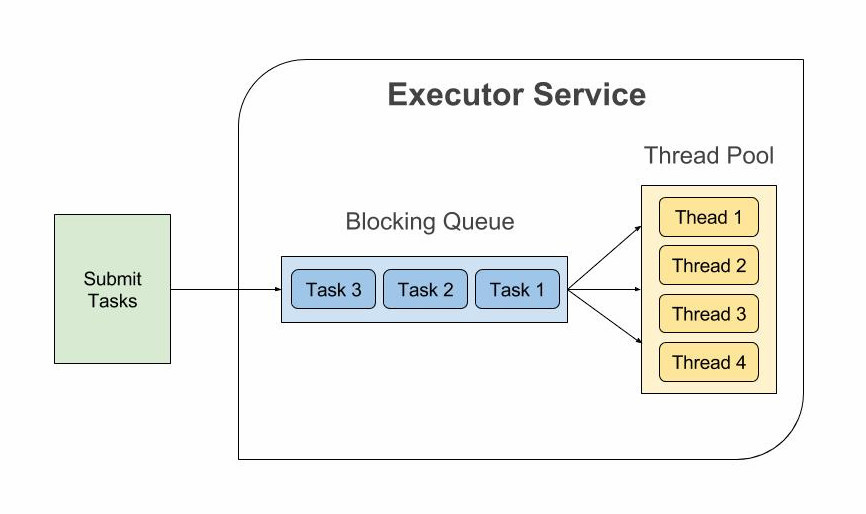
\includegraphics[width=.9\linewidth]{img/executor_service.jpg}

{\tiny Source: \url{https://www.callicoder.com/java-executor-service-and-thread-pool-tutorial/}}
\end{center}

\end{frame}

\subsection{Runnables}

\begin{frame}%[allowframebreaks]
\frametitle{Executing \texttt{Runnable}s -- Concept}

\begin{itemize}
\item Runnables can be \alert{executed} on an executor service by means of its \texttt{void execute(Runnable task)} method
\end{itemize}
%
\begin{center}
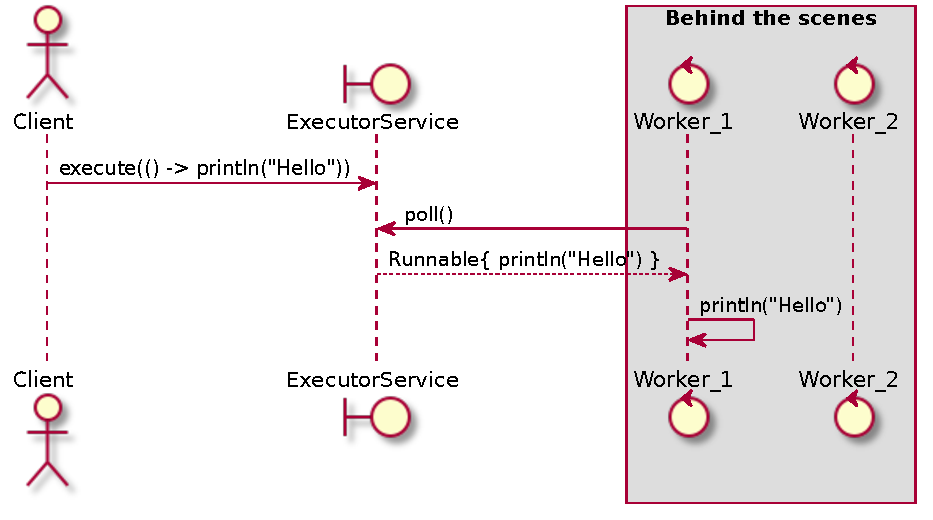
\includegraphics[width=.7\linewidth]{img/execute.pdf}
\end{center}
%
\hint{Notice that when the \texttt{execute()} method returns, the client has \alert{no guarantee} the task has \alert{already} been executed}

\end{frame}

\begin{frame}%[allowframebreaks]
\frametitle{Executing \texttt{Runnable}s -- Example}

\lstinputlisting{./code/execute_example.java}

\vfill

\begin{itemize}
\item \texttt{void shutdown()} prevents the executor service from accepting other tasks
\end{itemize}

\end{frame}

\begin{frame}%[allowframebreaks]
\frametitle{More examples on \texttt{ExecutorService}s}

Let's have a look to \href{https://gitlab.com/pika-lab/courses/ds/aa1920/lab-03/blob/master/src/test/java/sd/lab/concurrency/ExecutorServicesExamples.java}{\texttt{sd.lab.concurrency.\alert{ExecutorServicesExamples}}}

\vfill

\begin{block}{How to run a specific test in Gradle}
	\begin{itemize}
		\item[\$] \texttt{./gradlew cleanTest test --tests "test.class.package.\textit{TestClassName}.\alert{testMethodName}"}
	\end{itemize}
\end{block}

\vfill

\begin{block}{How to interpret a test for concurrent/asynchronous code}
	If you need to test the interaction among \alert{concurrent} control flows:
	\begin{enumerate}
		\item create a shared, ordered data structure, e.g. \texttt{List<\alert{Integer}>}
		
		\item let the many control flows add items to the data structure
		
		\item wait for all control flows to terminate
		
		\item draw assertions on the items content \& ordering from within the data structure
	\end{enumerate}
\end{block}

\end{frame}

\begin{frame}%[allowframebreaks]
\frametitle{Executing long-lasting, async computations -- Example}

\lstinputlisting{./code/AsyncCounter1.java}

\begin{itemize}
	\item[!] run tests in \href{https://gitlab.com/pika-lab/courses/ds/aa1920/lab-03/blob/master/src/test/java/sd/lab/concurrency/TestAsyncCounter1.java}{\texttt{sd.lab.concurrency.\alert{TestAsyncCounter1}}}
\end{itemize}

\end{frame}

\begin{frame}[c]
\frametitle{More examples on \texttt{ExecutorService}s \& \texttt{Runnable}s}

Consider having a look to the following examples as well
%
\begin{itemize}
	\item[!] \href{https://gitlab.com/pika-lab/courses/ds/aa1920/lab-03/blob/master/src/test/java/sd/lab/concurrency/SplittingComputationsExamples.java}{\texttt{sd.lab.concurrency.\alert{SplittingComputationsExamples}}}
\end{itemize}

\end{frame}

\subsection{Callables}

\begin{frame}[allowframebreaks]
\frametitle{Executing \texttt{Callable}s -- Concept}

\begin{itemize}
\item Callables can be \alert{submitted} on an executor service by means of its \texttt{Future<X> submit(Callable<X> task)} method

\vspace{.5cm}

% \begin{itemize}
\item The result of the asynchronous invocation can be retrieved by the caller by means of the returned \texttt{Future<X>} object
% \end{itemize}

\vspace{.5cm}

\item Futures represent \alert{placeholders} for results that will \emph{eventually} be(come) available
\end{itemize}
%
\framebreak
%
\begin{columns}
\begin{column}{.6\linewidth}
\begin{center}
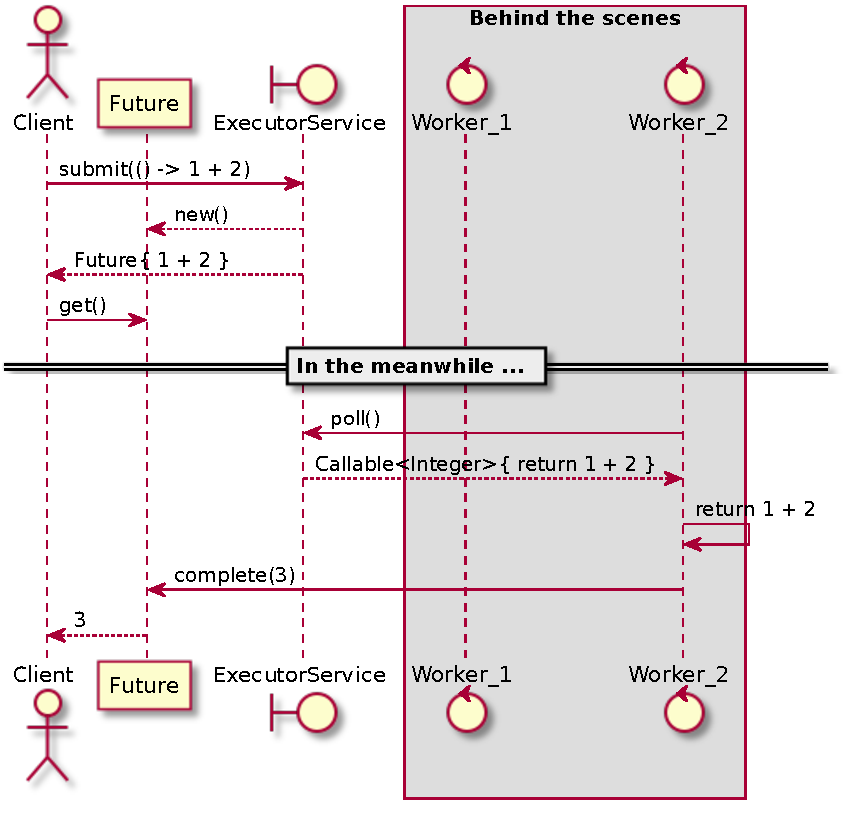
\includegraphics[width=\linewidth]{img/submit.pdf}
\end{center}
\end{column}
\begin{column}{.4\linewidth}
\begin{enumerate}
\item The client \alert{submits} a callable to an executor service

\item The executor service \alert{immediately} returns a future to the client

\item To retrieve the result, the client must invoke the \alert{\texttt{Future::get}} method

\item Such invocation \alert{blocks} until some worker thread actually computes the result

\end{enumerate}
\end{column}
\end{columns}

\end{frame}

\subsection{Futures}

\begin{frame}%[allowframebreaks]
\frametitle{The \texttt{Future} interface}

\lstinputlisting{./code/Future.java}

\begin{itemize}
	\item the blocking operation, i.e. \texttt{get}, is called \texttt{wait} or \texttt{\alert{await}} in other languages
	%
	\begin{itemize}
		\item and it is not always an instance method
	\end{itemize}
\end{itemize}

\end{frame}

\begin{frame}%[allowframebreaks]
\frametitle{Executing \texttt{Callables}s -- Example}

\lstinputlisting{./code/submit_example.java}

\end{frame}

\begin{frame}[c]
\frametitle{More examples on \texttt{Future}s}

Consider having a look to the following examples as well
%
\begin{itemize}
	\item[!] \href{https://gitlab.com/pika-lab/courses/ds/aa1920/lab-03/blob/master/src/test/java/sd/lab/concurrency/FuturesExamples.java}{\texttt{sd.lab.concurrency.\alert{FuturesExamples}}}
\end{itemize}

\end{frame}

\begin{frame}[allowframebreaks]
\frametitle{\texttt{CompletableFuture}s (a.k.a. Promises)}

\begin{itemize}
\item Futures are great for computing functions \alert{asynchronously}

\vspace{.3cm}

\item The examples presented so far, show how to create a future out of some Callable submission

\vspace{.3cm}

\item Can we explicitly decide which result should a future provide and when the caller should be unlocked?

\vspace{.6cm}

\item[$\rightarrow$] \texttt{\alert{CompletableFuture}}s (or Promises) are what we need: they come with a \texttt{boolean complete(X value)} method which can be called within tasks
\end{itemize}

\framebreak

\lstinputlisting{./code/CompletableFuture.java}

\end{frame}

\subsection{CompletableFutures}

\begin{frame}%[allowframebreaks]
\frametitle{\texttt{CompletableFuture}s (a.k.a. Promises) -- Example}

\lstinputlisting{./code/AsyncCounter2.java}

\end{frame}

\begin{frame}%[allowframebreaks]
\frametitle{\texttt{CompletableFuture}s -- Client side}

\lstinputlisting{./code/AsyncCounter2Test.java}

\end{frame}

\begin{frame}[c]
\frametitle{More examples on \texttt{CompletableFuture}s}

Consider having a look to the following examples as well
%
\begin{itemize}
	\item[!] \href{https://gitlab.com/pika-lab/courses/ds/aa1920/lab-03/blob/master/src/test/java/sd/lab/concurrency/TestAsyncCounter2.java}{\texttt{sd.lab.concurrency.\alert{TestAsyncCounter2}}}
	\item[!] \href{https://gitlab.com/pika-lab/courses/ds/aa1920/lab-03/blob/master/src/test/java/sd/lab/concurrency/PromisesExamples.java}{\texttt{sd.lab.concurrency.\alert{PromisesExamples}}}
\end{itemize}

\end{frame}

\section{Check your understanding}

\begin{frame}[c]
\frametitle{Exercise 3-1: \texttt{AsyncCalculator} I}

Consider the \href{https://gitlab.com/pika-lab/courses/ds/aa1920/lab-03/blob/master/src/main/java/sd/lab/concurrency/exercise/AsyncCalculator.java}{\texttt{sd.lab.concurrency.exercise.\alert{AsyncCalculator}}} interface:
%
\vfill
%
\lstinputlisting{./code/AsyncCalculator.java}
%
\vfill
%
\begin{enumerate}
	\item Provide an implementation for such an interface\ldots
	
	\vfill
	
	\item \ldots in such a way that tests in \href{https://gitlab.com/pika-lab/courses/ds/aa1920/lab-03/blob/master/src/test/java/sd/lab/concurrency/exercise/TestAsyncCalculator.java}{\texttt{sd.lab\allowbreak{}.concurrency\allowbreak{}.exercise\allowbreak{}.\alert{TestAsyncCalculator}}} are all satisfied
\end{enumerate}

\end{frame}

\begin{frame}[c]
\frametitle{Exercise 3-1: \texttt{AsyncCalculator} II}

\begin{enumerate}\setcounter{enumi}{2}
	\item Submit your exercise to the following branch on Lab 3 repository
	%
	\begin{center}
		\texttt{submissions/\textit{name.surname}}
	\end{center}

	\vfill

	\item Continuous Integration will automatically run tests
\end{enumerate}

\end{frame}


%===============================================================================
\section*{}
%===============================================================================

%\\\\\\\\\\\\\\\\\\\\\
\frame{\titlepage}
%\\\\\\\\\\\\\\\\\\\\\

%%===============================================================================
%\section*{\refname}
%%===============================================================================
%
%%\\\\\\\\\\\\\\\\\\\\\
%%%%%
%%\begin{frame}[t,allowframebreaks]\scriptsize
%\begin{frame}[c]\footnotesize
%\frametitle{\refname}
%\bibliographystyle{apalike}
%\bibliography{sd-lab-async-programming}
%\end{frame}
%%\\\\\\\\\\\\\\\\\\\\\

%%%%%%%%%%%%%%%%%%%%%%%%%%%%%%%%%%%%%%%%%%%%%%%%%%%%%%%%%%%%%%%%%%%%%%%%%%%%%%%
\end{document}
%%%%%%%%%%%%%%%%%%%%%%%%%%%%%%%%%%%%%%%%%%%%%%%%%%%%%%%%%%%%%%%%%%%%%%%%%%%%%%%%

